\documentclass[12pt]{article}
\usepackage[margin=1in]{geometry}
\usepackage{mlmodern}
\usepackage{array}
\usepackage{amsmath, amssymb, amsfonts}
\usepackage{pgfplots}
\usepackage{graphicx}
\pgfplotsset{compat=1.18, width=10cm}

\pagestyle{empty}
\parindent 0px
\title{Taylor Series}
\author{Hamza Kamal}
\date{\today}

\newcommand{\formula}[2]{
    {\renewcommand{\arraystretch}{2}
        \begin{center}
        \begin{tabular}{|p{0.9\textwidth}|}
        \hline
        \textbf{#1} \\
        \hline
        #2 \\
        \hline
        \end{tabular}
        \end{center}
    }
}

\begin{document}

\setlength{\jot}{10pt}

\begin{titlepage}
\maketitle
\thispagestyle{empty}
\end{titlepage}

\tableofcontents
\newpage

\section{Prerequisites: }

\subsection{Taylor Series Approximation: }
The approximated expansion for the Taylor Series of the function $f(x)$ centered at $x=a$ is given by the following formula:
\formula{Taylor Series Approximate Expansion}{$f(x) = f(a) + f'(a)(x-a) + \frac{f''(a)}{2!}(x-a)^2 + \frac{f'''(a)}{3!}(x-a^3 + \ldots)$}
Where each constant is represented by an increasing derivative of the function $f(x)$ at some value $a$.

\subsection{Linear Approximation: }
Linear approximation, also known as linearization or tangent line approximation, is a method used in calculus to estimate the value of a function near a specific point by using the equation of the tangent line at that point. The linear approximation provides a good approximation of the function's behavior in the vicinity of the chosen point.
\vspace{\baselineskip}
The linear approximation is based on the idea that a sufficiently smooth and well-behaved function can be approximated by a linear function (a straight line) near a particular point. The equation of the tangent line to the graph of the function at a given point $(a, f(a))$ is given by:
\formula{Linear Approximation}{$L(x) = f(a) + f'(a)(x - a)$}
Here:
\begin{itemize}
  \item $L(x)$ is the linear approximation to the function,
  \item $f(a)$ is the value of the function at the point $x = a$,
  \item $f'(a)$ is the derivative of the function evaluated at $x = a$,
  \item $x$ is the variable.
\end{itemize}
\subsubsection{Example: }
Find the value of $\sqrt{4.3}$ using the function $f(x)=\sqrt{x}$.

\vspace{\baselineskip}
In this case the closest whole number that the function $f(x)$ outputs is $f(4) = \sqrt{4}$ which equals $2$. So, our $a = 4$, $f(a)=2$ and $f'(a)= \frac{1}{2\sqrt{4}}$ which is $\frac{1}{4}$.

\vspace{\baselineskip}
Therefore, our equation of the tangent line is $L(x) = f(a) + f'(a)(x - a) = 2 + \frac{1}{4} (x-4)$. Plugging in $L(4.3)$ we get that $\sqrt{4.3} \approx 2.075$.

\subsection{Absolute Value Equations: }
\formula{Absolute Value Function}{$|x| = \begin{cases} x & \text{if } x \geq 0 \\ -x & \text{if } x < 0 \end{cases}$}
The absolute value function $|x|$ returns the non-negative distance of $x$ from zero on the number line.
\formula{Absolute Value Equation}{$|f(x)| = g(x)$}
Absolute value equations relate the absolute value of an expression $f(x)$ to another expression or constant $g(x)$.
\textbf{Solving Procedure:}
\begin{enumerate}
    \item Solve \(f(x) = g(x)\)
    \item Solve \(f(x) = -g(x)\)
\end{enumerate}
Solving each case may yield two sets of solutions, and validity is checked by substitution into the original equation.

\subsubsection{Example: }
Solve $|2x - 5| = 7$.
\begin{enumerate}
    \item \textbf{Isolate the Absolute Value Expression:}
    $2x - 5 = 7$ or $2x - 5 = -7$
    \item \textbf{Apply the Absolute Value Property:}
    $2x = 12$ or $2x = -2$
    \item \textbf{Solve for the Variable:}
    Solutions: $x = 6$ and $x = -1$.
    \item \textbf{Check for Extraneous Solutions:}
    Both solutions are valid.
\end{enumerate}

\section{Power Series: }
A power series is an infinite series with the form:
\formula{Power Series}{$\sum_{k=0}^{\infty} c_k x^k = c_o + c_1 x + c_2 x^2 + \dotsc + c_n x^n + c_{n+1} x^{n+1} + \dotsc$}

This power series is centerd at $0$. The more general formula that includes power series centered at $a$ is:
\formula{Power Series}{$\sum_{k=0}^{\infty} c_k (x-a)^k = c_o + c_1 (x-a) + c_2 (x-a)^2 + \dotsc + c_n (x-a)^n + c_{n+1} (x-a)^{n+1}$}

\section{Taylor Polynomials: }
Let $f$ be a funcion with $f', f'', \dotsc, f^{(n)} $ defined at $a$. The \textit{nth} order Taylor Polynomial $p'$ for $f$, centered at $a$, matches $f$ in value, slope, and all derivatives up to the \textit{nth} order at $a$.
\formula{Taylor Polynomials}{}

\section{Binomial Series: }
\textbf{Binomial Definition:}
The term "binomial" is derived from the Latin words "bi" which means two and "nomen" which means name. Which shows that binomials involve expressions with two terms, for example: $(a+b)$.

Here are some examples of binomials:
\begin{gather*}
(1+x)^0 = 1 \\
(1+x)^1 = 1+x \\
(1+x)^2 = 1 + 2x + x^2 \\
(1+x)^3 = 1 + 3x + 3x^2 + x^3 \\
(1+x)^4 = 1 + 4x + 6x^2 + 4x^3 + x^4
\end{gather*}

This pattern is derived from Pascals Triangle which lists out the coefficients for each term.

\begin{figure}[h]
\centering
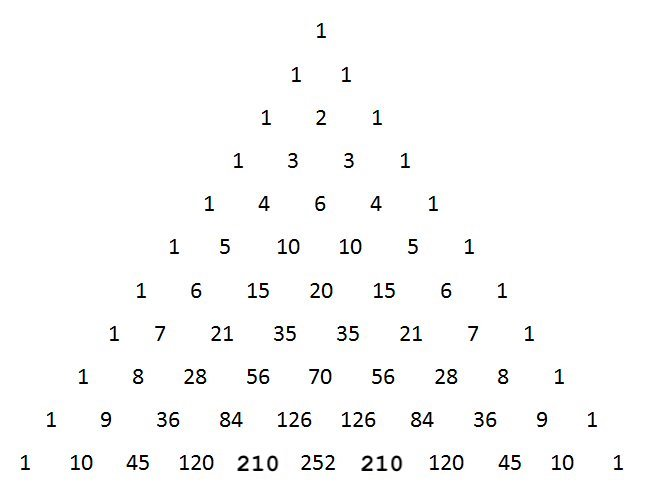
\includegraphics[width=0.6\textwidth]{img/pascals_triangle}
\caption{Pascals Triangle}
\end{figure}

\newpage

However, if we wanted to calculate larger and larger powers of $(1+x)$ you can see that this would become difficult and cumbersome. For example if you wanted to calculate $(1+x)^n$ where $n$ was a very large value like $8$ it would not be wise to write out $8$ rows of Pascals Triangle and then find the coefficients to write the answer.

We have a name for the terms that appear in the Pascals Triangle which are also the powers $(1+x)$. We call them \textit{binomial coefficients}.

\formula{Binomial Coefficients}{$\binom{p}{k} = \frac{p!}{k!(p-k)!}$}
Note: The numbers $\binom{p}{0}, \binom{p}{1}, \binom{p}{2}, \dotsc, \binom{p}{p}$ form the "$p$th" row on the Pascals Triangle.

\vspace{\baselineskip}

More generally, if $p$ is any real number and $k >= 1$ is an integer, then:

\formula{Binomial Coefficients}{$\binom{p}{k} = \frac{p(p-1)(p-2)\dotsc(p-k+1)}{k!}$}

The Special Symbol $\binom{p}{k}$ is pronounced "p choose k".

\subsection{Examples: }

\subsubsection{Example 1: }
If you had a class of 30 students and you had to pick a team of 3 students. This would be "30 choose 3" or $\binom{30}{3}$.
\begin{gather*}
\binom{30}{3} = \frac{30!}{3!(27)!}
\end{gather*}
You can solve this equation to get the answer to the problem.
\vspace{\baselineskip}

\subsubsection{Example 2: }
What if we wanted to find the 8th row of Pascals Triangle.
\vspace{\baselineskip}
This would be the same as doing: $\binom{8}{0} = 1, \binom{8}{1} = \frac{8!}{1!(7)!}, \binom{8}{2} = \frac{8!}{2!(6)!}, \dotsc, \binom{8}{n} = \frac{8!}{n!(8-n)!}$
\vspace{\baselineskip}
Solving this you can calculate $(1+x)^8$ which equals $1 + 8x + 28x^2 + 56x^3 + 70x^4 + 56x^5 + 28x^6 + 8x^7 + x^8$.
\vspace{\baselineskip}

\subsubsection{Example 3: }
Find $\binom{-3}{2}$ and $\tbinom{\frac{1}{2}}{3}$.
$$\binom{3}{-2} = \frac{-3(-3-1)}{2!}$$
Because $k=2$ there are only $2$ factors on the top $-3(-3-1)$.
\begin{gather*}
\binom{3}{-2} = \frac{-3(-3-1)}{2!} \\
= \frac{(-3)(-4)}{2} \\
= 6
\end{gather*}
$$\binom{\frac{1}{2}}{3} = \frac{\frac{1}{2} (\frac{1}{2} - 1) (\frac{1}{2} - 2)}{3!}$$
Because $k=3$ there are only $3$ factors on the top $\frac{1}{2} (\frac{1}{2} - 1) (\frac{1}{2} - 2)$
\begin{gather*}
\binom{\frac{1}{2}}{3} = \frac{\frac{1}{2} (\frac{1}{2} - 1) (\frac{1}{2} - 2)}{3!} \\
= \frac{\frac{1}{2} (\frac{-1}{2}) (\frac{-3}{2})}{6} \\
= \frac{\frac{3}{8}}{6} \\
= \frac{1}{16}
\end{gather*}

\formula{Binomial Series}{$\sum_{k=0}^{\infty} \binom{p}{k}x^k = 1 + \sum_{k=1}^{\infty} \frac{p(p-1)(p-2) \dotsc (p-k+1)}{k!}x^k$}

\end{document}